%%%%%%%%%%%%%%%%%%%%%%%%%%%%%%%%%%%%%%%%%%%%%%%%%%%%%%%%%%%%%%%%%%%%%%
%
%  Epigenetic Robotics 2006
%
%  We are using SAB format.
%  Choose  'a4' for your draft.
%  (Note that the final proceedings will be using A4 paper.)

\documentclass[a4]{epirob}

%  usepackage goes here.

\usepackage{graphicx}

%%%%%%%%
%
%  title/author/affiliation go here.
%  Note: we slightly changed the use of author/affilication.
\title{A sensitive approach to grasping}

%
%  For one-to-one authur/affil correspondence

%\author{Lorenzo Natale\\
%   \rm  Massachusetts Institute of Technology\\
%   \rm  Computer Science and Artificial Intelligence Laboratory\\
%   \rm  32 Vassar St. Room 32-380\\
%   \rm  Cambridge, MA 02139 US\\
%   \rm  lorenzo@csail.mit.edu
%  \and
%        Eduardo Torres-Jara\\
%   \rm  Massachusetts Institute of Technology\\
%   \rm  Computer Science and Artificial Intelligence Laboratory\\
%   \rm  32 Vassar St. Room 32-380\\
%   \rm  Cambridge, MA 02139 US\\
%   \rm  etorresj@csail.mit.edu}
%
%\affiliation{} % not used in one-to-one mode

%
%  For N-to-M author/affil correspondence
%
  \author{Lorenzo Natale$^{*}$$^{\dag}$\\
          \rm  lorenzo@csail.mit.edu
        \and
          Eduardo Torres-Jara$^{*}$\\
          \rm  etorresj@csail.mit.edu}
  \affiliation{$^{*}$Massachusetts Institute Technology\\
    \rm  Computer Science and\\
    \rm Artificial Intelligence Laboratory\\
    %\rm  CSAIL\\
    \rm  32 Vassar St. Room 32-380\\
    \rm  Cambridge, MA 02139 US\\
             \and
              $^{\dag}$\rm  University of Genoa\\
   \rm  LIRA-Lab, DIST\\
   \rm  Viale F. Causa 13\\
   \rm  16145 Genoa, Italy
   }

%%%%%%%%
%
%  Local setting (if any) goes here.

%  Now, let us begin.

\begin{document}

\maketitle

\begin{abstract}
Experimental results in psychology have shown the important role
of manipulation in guiding infant development. This has inspired
work in developmental robotics as well. In this case, however, the
benefits of this approach has been limited by the intrinsic
difficulties of the task. Controlling the interaction between the
robot and the environment in a meaningful and safe way is hard
especially when little prior knowledge is available. We push the
idea that haptic feedback can enhance the way robots interact with
unmodeled environments. We approach grasping and manipulation as
tasks driven mainly by tactile and force feedback. We implemented
a grasping behavior on a robotic platform with sensitive tactile
sensors and compliant actuators; the behavior allows the robot to
grasp objects placed on a table. Finally, we demonstrate that the 
haptic feedback originated by the interaction with the objects carries
implicit information about their shape and can be useful for learning.
\end{abstract}
\section{Introduction}
Growing evidence in developmental psychology shows the importance 
of motor activity for cognitive development in humans \cite{gallese06mirror}. 
In particular it is through manipulation that infants gain direct access to objects 
and discover properties that otherwise would remain hidden. 
This concerns for example properties like weight, shape, texture and 
softness that are, if not impossible, at least extremely hard to perceive 
by using visual information alone. In adults information originating 
from motor activity and direct contact with the environment, supports 
perception \cite{klatzky87hand}; during development
the physical interaction with the environment provides infants 
with natural invariances that are useful occasions for learning.
Interestingly, motor and perceptual development seem to follow synchronous  
schedules as if new achievements in the motor system were promoting
the development of new perceptual skills \cite{bushnell93motor}.

Research in developmental robotics has demonstrated the importance of
motor activity (in particular manipulation) for visual and haptic 
perception \cite{fitzpatrick07shared}. One of the 
limitations of these approaches is that controlling the interaction between
the robot and the environment is difficult especially when precise models are
not available. Experiments with robots have thus focused on situations
in which the interaction with objects is relatively simple. For these reasons
the investigation of perceptual development in robots requires addressing 
the problem of motor development first and improving how robots interact
with the world.

In this context we focus on reaching, which is clear prerequisite for 
grasping. If vision of the hand and target were available then this problem 
would be easily solved by employing a visual servoing approach (see 
\cite{hutchinson96tutorial} for a review) which is typically based on 
the use of the visuo-motor Jacobian of the arm. The eye-to-hand Jacobian 
transformation is a function of the arm and head joints and includes knowledge 
of the camera parameters; its estimation is in practice a difficult task.
The fundamental advantage of this approach is that even an inaccurate estimation 
of the Jacobian allows reducing the error of the task to zero. But the visual 
servoing approach is not necessarily the best solution. On one hand delays in 
the control loop pose limitations on the speed of the arm, while on the other 
hand it requires that the hand and target are continuously visible for the 
duration of the movement. 
Reaching can also be performed open-loop by directly relating the joint angles of 
the head with those of the arm \cite{blackburn94learning,metta99developmental}. 
The drawback of this approach is that errors because of modeling inaccuracies and 
noise in the sensors, calculations, actuation, cannot be made arbitrarily small 
as in the visual servoing case.

Results in developmental psychology suggest that both solutions might be
adopted by the brain. Clifton et al. \cite{clifton93isvisually} 
tested whether infants require vision of their hand when reaching; they 
found that infants' ability to touch (and grasp) objects is independent 
of whether sight of the hand is available or not. On the other hand 
other experiments \cite{ashmead93visual} show that later on in development 
there is an increase of visual guidance in reaching. Together these results 
suggest the hypothesis that there are two ``distinct'' reaching mechanism: 
one that relies on ``proprioceptive'' information alone and one that uses 
``visual feedback'' to compensate for errors in the visual domain. Further,
there are studies that show the link of the control of the gaze in relation
to the precision of reaching \cite{flanders-daghestani-berthoz-1999}. 
In this paper we integrate the two modes of control with an approach based on
the hypothesis that the target object is fixated. We use the open loop
controller to bring the hand close to the target. The closed loop controller 
is activated when visual feedback from the hand is available. In practice,
we show that the error could be made arbitrarily small. The problem of 
redundancy in solved in the first case by imposing additional constraints to 
the task. Finally, we describe the procedure by which the robot learns all 
the transformations required by the controllers (the open-loop mapping and 
the arm visual Jacobian).
\section{Background}
\label{sec:background}

The tactile sensing in neonates is very poorly known
 in contrast to the visual mechanism\cite{Streti-voir-atteindre-toucher}.
However, tactile sensing provides information to children since
his time in the wound. Hands and arms are intensively used to
learn about their environment even though their motion
capabilities are not completely developed at an early stage.
Moreover, some experiments suggests that in some circumstances
children learn about the objects by tact only, leaving out vision.
For example, \cite{StretiHabituation} placed different objects in
the hand of children who had no visual contact with their hand.
The time that the children hold the object was used to determine
when they habituated to the object. After hand in the object a
number of times the holding time is reduced. When new objets where
presented the holding time increased. This shows learning and
adaptation to novelty. This experiment was repeated with visual
feedback showing the same behavior.
% As shown in the experiment: a
%3D projection of an object was shown to children form....
Integration between the visual and tactile modalities also occurs
at early stages. Tactile information is, for example, used to
confirm visual stimulus as described in the following experiment
\cite{tactileconfirmation}. An image of an object was projected
used polarized lenses so that children wearing ``stereo'' glasses
perceived a 3D object. The children reacted surprised when they
tried to reach it but did not feel the contact when expected. The
children ages were between 6 days to 6 months. Children up to 4
months closed their hand when they were expecting the contact. The
older ones remain with the hand open.

In adults, several studies have revealed the importance of
somatosensory input (force and touch). For example
\cite({Johansson90Liffiing, has studied in detail what feedback
the skin provides to the task of lifting an object and how it is
used to control the movements of the fingers. Highlighting the
importance of this information when human subjects were
anesthetized their fingertips, they have difficulties applying the
right forces to avoid slipping when lifting an object with full
vision (Johansson, 1991).

%Tactile sensing gets information from the object and triggers
%motor responses. This is because the mechanoreceptors, being
%closer to manipulate the object, provide timely mechanical
%information of the interaction between the hand and the
%object\cite{Johansson90Liffiing}. In \cite{Johansson90Liffiing} an
%analysis of the forces observed in the grasp-and-lift task is
%presented. The analysis of many transition phase is mentioned but
%not much data is provided about the initial contact. Which is a
%big problem in robotics\cite{volpe90real}.

Humans use a set of strategies collectively called exploratory
procedures (Lederman and Klatzky, 1987) in their perception of the
world around them, such as tracing object outlines with a finger.
%This has inspired work on robotics.

We address the task of approaching and lifting an object using
tactile feedback to modulate the motor control of the hand and the
arm.


%In robotics exploratory robotics has been developed to do the
%same. Active exploration is needed in unstructured environments.
%(Bajcsy 1989). Humans are very good at extracting propreties of 3D
%objects. Very bad at 2-D compared to Vision. (cite).



%An analog of human sensitivity to thermal diffusivity was
%developed by (Campos et al., 1991), allowing a robot to
%distinguish metal (fast diffusion) from wood (slow diffusion).

%Tactile information gets information from the object and triggers
%motor responses. This is because the mechanoreceptors, being
%closer to manipulate the object, provide timely mechanical
%information of the interaction between the hand and the
%object\cite{Johansson90Liffiing}. In \cite{Johansson90Liffiing} an
%analysis of the forces observed in the grasp-and-lift task is
%presented. The analysis of many transition phase is mentioned but
%not much data is provided about the initial contact. Which is a
%big problem in robotics\cite{volpe90real}.


%Infromation of the tactile sensors during manipulative finger
%movements and its utilization in motion control. Known in flexing
%movements of teh receptor-bearing fingers.

%\cite{Johansson90Liffiing} states the importance of teh teactile
%feedback in the motion control of hand. Tactile feedback afferents
%resopnd during mnaipulative tasks (suach lifting). These
%activation are important for the control of manipulation.





%Experimental results suggest that from a very early age, arm
%movements in infants are influenced by vision. For example, van
%der Meer and colleagues found that sight of the hand allows
%infants to maintain the posture of the hand when pulled by an
%external force (van der Meer et al., 1995). Von Hofsten compared
%the arm movements of two groups of infants in the presence and
%absence of an object and found that in the former case arm
%movements were significantly more frequent. When the infants were
%fixating the objects the movements were directed closer to it (von
%Hofsten, 1982). Taken together, these results suggest that in
%children some sort of eye-hand coordination is already present
%soon after birth. But on the other hand, continuous visual
%feedback from the hand is not required for infants to reach for an
%object (Clifton and D.W. Muir, 1993, Clifton et al., 1994). Indeed
%it is only at 9 months of age that children seem to be able to
%exploit visual feedback from the hand during the approach phase
%(Ashmead et al., 1993). A possible explanation for this could be
%that in the first months of development the visual system of
%infants is still rather immature: visual acuity is limited and
%perception of depth has not developed yet (Bushnell and Boudreau,
%1993). Later on during development the role of vision is certainly
%crucial to control the correct preshape of the hand according to
%the object's shape and orientation; however, tactile feedback from
%the contact with an object is an alternative source of information
%that could initially substitute for the visual feedback. In
%adults, several studies have revealed the importance of
%somatosensory input (force and touch); for example human subjects
%with anesthetized fingertips have difficulty in handling small
%objects even with full vision (Johansson, 1991). Humans use a set
%of strategies collectively called exploratory procedures (Lederman
%and Klatzky, 1987) in their perception of the world around them,
%such as tracing object outlines with a finger. This has inspired
%work on robotics. An analog of human sensitivity to thermal
%diffusivity was developed by (Campos et al., 1991), allowing a
%robot to distinguish metal (fast diffusion) from wood (slow
%diffusion).

%The importance of interacting with the world to learn form it has
%been repeatly stated. .. The development of the hand-eye
%coordination has been reported as important for adquiring ... and
%for interacting in the world.


%Contact with objects to extract properties is important. However,
%actual contact with the world has been limited in robotics.
%\cite{volpe90real}, for example, has analyzed the problem of
%impact. That is the first contact were usually the robot switches
%form force control to position control and inestabilyt can be
%presetn. Especailly becaus teh impact produces oscillation that
%make the robto  to operate between the condition s of contact and
%not contact withte table. This nono-linearity makes even more
%possible the inestability.






%In adults, several studies have revealed the importance of
%somatosensory input (force and touch); for example human subjects
%with anesthetized fingertips have difficulty in handling small
%objects even with full vision(Johansson, 1991). Humans use a set
%of strategies collectively called exploratory procedures (Lederman
%and Klatzky, 1987) in their perception of the world around them,
%such as tracing object outlines with a finger. This has inspired
%work on robotics. An analog of human sensitivity to thermal
%diffusivity was developed by (Campos et al., 1991), allowing a
%robot to distinguish metal (fast diffusion) from wood (slow
%diffusion).

%Skin feedback has not been considerd in  conotrol, for example the
%possible feedback of postion no  joints.

\section{The robot Obrero}
\label{sec:platform}

Obrero \cite{obrero} 
consists of a hand, an arm and a head (Figure~\ref{fig:RobotObrero}). 
Obrero was designed to approach manipulation as a task manly guided by
tactile and force feedback.
We use the robot's limb as a sensing/exploring device as opposed 
to a pure acting device. This is a convenient approach to operate 
in unstructured environments, on unmodeled objects. 
Obrero's limb is sensor-rich and
safe, it is designed to reduce the risk of damages upon contact
with objects. The head consists of a commercial camcorder (SONY) 
that can move along the pan and tilt directions. The arm has 6 
Degrees of Freedom (DOF) distributed in this way: 3 in the shoulder, 1 at the level of 
the elbow and 2 in the wrist. The arm mounts Series Elastic Actuators 
\cite{williamson95series} which provide low-impedance and force feedback 
at each joints (\cite{domo}). Position feedback is provided by 
analog encoders (potentiometers).

The hand consists of a palm, a thumb, a middle and an
index finger. Each one of the fingers has two links that can be
opened and closed. The thumb and the middle finger can also
rotate. These rotations allow the the thumb to oppose to either 
the index or the middle fingers.

%By rotating the thumb it can be opposed to the index
%finger and by rotating the thumb and the middle, they can oppose
%to each other.

The total number of degrees of freedom in the hand is 8. The hand 
is underactuated, only 5 motors are connected to the fingers. Three motors control
the opening and closing of the fingers. The remaining two motors actuate
the rotation of the thumb and middle finger. The phalanges in each fingers 
are mechanicaly coupled and actuated by a common motor. The link between 
the two joints is realized by means of Series 
Elastic Actuators, to allow independent motion 
whenever one of the phalanges blocks (for example as a result of contact 
with an object). This elastic coupling allows the hand to automatically 
adapt to the object it grasps. All joints in the hand are equipped with an 
optimized version of the Series Elastic Actuators \cite{actuator} which provide 
force feedback and reduce the mechanical impedence of the fingers. Finally 
position feedback is obtained through analog encoders mounted in all joints. 

%However, they can decouple thanks to the SEA's in each
%joint. All the joints of the hand are controlled using an
%optimized design for a series elastic actuator \cite{actuator}.
%There are a total of 8 SEA's int the hand. Series elastic
%actuators\cite{williamson95series} reduce their mechanical
%impedance and provide force sensing.

The tactile sensors mounted on the robot were designed for robotic tasks. 
Their design was inspired by the dome-like shape of the ridges that have been 
observed in the human skin, where, the innervations at the base of the ridges 
detect the deformation of the skin. 

Inspired by this mechanism we realized a tactile sensor made of silicon rubber 
and with a dome-like shape (see figure\ref{}). At the tip of the dome, in the 
internal part, we mounted a small magnet, whose position is measured by four 
hall-effect sensors placed at the base. The hall-effect sensors in this way 
measure the deformation of the dome by sensing the position of the magnet at the 
tip. The sensors are very sensitive and have been tested to detect up to the 
minimum normal force of 10g. 

The shape the sensors favors contact with the environment from any direction, 
as opposed to most of the tactile sensors which are flat. 
This high deformability and the properties of the silicon rubber allow the 
sensors to conform to the objects, thus increasing friction and improving 
contact detection. 

In the particular implementation used in this paper, we used the ``magnetic'' 
version of the tactile sensors, however, a optical version has been also tested. 
An analysis and description of the design of these sensors can be
found in \cite{etorresjSoft}. Groups of tactile sensors were
placed in parts of the hand. Two groups of four
were placed on each finger (a group in each of the two falanges)
and 16 on the palm. A detail of the palm and fingers can be
observed in figure\ref{}. Each one of these tactile sensors uses 4
sensors to determine the contact forces. That means that overall the 
tactile feedback consist of 160 sensors. At the base of the
palm, where for practical reasons, we were not able to mount 
these tactile sensors, we placed a smaller infrared proximity sensor. 
To summarize, the hand has 5 motors, 8 DOF, 8 force sensors, 10 position
sensors, 160 tactile sensors and a infrared proximity sensor.


\section{Overall developmental approach}
 \label{sec:approach}
[Should we keep this??]

 We wish to give our robots many ways to learn about
objects through action (Fitzpatrick et al., 2003). This
contributes to perceptual development, where the robot's
experience of the world is filtered by prior experience. This
process can be broken down into four steps:

\begin{itemize}

\item Identification of an opportunity to reliably extract some
object features.

\item Exploitation of that opportunity to extract those features.

\item Use careful generalization to transform the robot's
perception of its environment.

\item Transformation of the robot's activity, enabled by its
extended perceptual abilities.

\end{itemize}

In previous work, we have demonstrated this process. In (Arsenio
et al., 2003), we showed that poking an object gives us the
opportunity to reliably extract visual features of its appearance.
By carefully choosing features that generalize, the robot's
perception of its environment is transformed, and new activities
are enabled (Fitzpatrick, 2003b). Other opportunities we have
explored include the use of grasping (Natale et al., 2005) and the
integration of multi-modal cues across sound, vision, and
proprioception (Fitzpatrick et al., 2005, Arsenio and Fitzpatrick,
2005). Having established this process, we are now seeking to
broaden the range of opportunities that can be identified and
exploited (steps 1 and 2 above). In the current work, we identify
(and in fact create) an opportunity to reliably extract examples
of contact sounds involving an object (by tapping that object). We
build the appropriate robot behavior and data collection
infrastructure to gather those features.

\section{Controlling the body}
\label{sec:controlling}
%
In this section we describe a few perceptual and motor competencies required
for the robot to be able to control the body in a meaningful and safe way:
this includes a simple attention system to spot the objects to be grasped
and the ability to control the body to reach out for them. A the end of the
section we describe how the these capabilities are integrated in the grasping
behavior.
%
\subsection{Attention System}
Motion is a simple yet powerful cue to select points of interest
in the visual scene; for an active camera system this is still
true assuming we can estimate the motion of the background and
account for it. In this paper we use the algorithm proposed by
\cite{kemp-thesis}, which uses a 2D affine model to robustly
estimate the image motion resulting from the background. In short,
the algorithm measures the motion of each pixel with a block
matching procedure, and performs a least square fitting of the
global affine model. Using the affine model the algorithm predicts
the motion of each edge, and marks as foreground
those edges that poorly match this prediction. Under the
assumption that the majority of the image motion is due to the
background, these edges can be used to build a saliency map to
direct the attention of the robot.
%
\subsection{Eye-hand coordination}
We decided to focus on explorative
actions rather than precise, goal directed, actions towards the target objects.
This was also motivated by the fact that the monocular visual system of Obrero
makes depth estimation very difficult. This situation is actually quite common
in robotics, as depth estimation in real time is a challenging problem even 
with stereo vision.
However, we cannot hope to program the robot to perform
a blind exploration of the entire workspace. A possible solution is to
constrain the exploration to the area of the workspace where the object is
detected visually. Since the 3D location of the object is not available, 
reaching is performed in 2D; the exploration procedure allows the 
robot to find the actual position of the object. The motor skills 
required for reaching and exploring can be learned from the 
visual ability to localize the hand and compute the 
orientation of the arm.
%
\subsection{Hand Localization}
A visual module detects the hand and computes the orientation of
the arm in the image. The initial step of the hand detector
consists in running a high frequency filter. All points whose
frequency is below a certain threshold (fixed a priori) are
discarded. A blob detector is run on the resulting image and the
biggest blob is selected as the arm. The orientation of the arm is
computed as the orientation of the line passing through the
top-most and bottom-most pixels of the arm area. Next, specific
features (the small circular black and white potentiometers on the
fingers) are searched on the arm area. The hand is identified if
more than two of these features are found. The detection just
described proved reliable enough for our purposes and was used as
a short-cut in place of other, more general, methods
\cite{metta03early,natale05from}.

The visual feedback of the hand could be used for closed-loop control.
However closed-loop control is not always suitable. This happens for example
in presence of occlusions or when the hand is not within the visual field.
%
Open-loop control is an alternative solution. A possible open-loop
control consists of a mapping between the fixation point of the
head and the arm end-point \cite{metta00Babybot}. The advantage of
this approach is that the mapping can be easily learned if the
robot is able to look at the hand. Another approach uses the output of the 
hand detector to learn a direct mapping between the arm
proprioception (encoder feedback) and the position of the hand in
the image \cite{natale05from}. The direct (forward) mapping
can be inverted locally to control the arm to reach for a visually
identified target. The solution we adopt here is similar: in a
discovery phase the robot tracks the hand as the arm moves to
randomly explore the workspace. This behavior allows the robot to
acquire samples in the form:
%
\begin{center}
\begin{math}
  \left(\begin{array}{ccccc}
    x & y & \alpha &q_{head} &q_{arm} \end{array}\right)_{0,1\dots,k}
\end{math}
\end{center}
%
where $x$, $y$ and $\alpha$ are the coordinates of the hand and the 
orientation of the arm in the image, $q_{head}$ and $q_{arm}$ are
the position of the head and arm respectively. Given $q_{head}$ it is
possible to convert $x$ and $y$ into an egocentric reference frame:
%
\begin{equation}
  \left[
  \begin{array}{ccc}
    \theta_h & \phi_h
    \end{array}\right]^T
  = f_{head}^{-1}
  \left(\left[\begin{array}{ccc}
    x &
    y &
    q_{head}
    \end{array}\right]^T \right)
\label{eq-head-inverse}
\end{equation}
%
$\theta_h$ and $\phi_h$ represents the polar coordinates of the hand in the
reference frame centered at the base of the head (azimuth and elevation). 
Basically $f_{head}^{-1}$ includes knowledge of the inverse kinematics of the
head and the parameters of the camera. The opposite transformation maps
polar coordinates into the image plane:
\begin{equation}
  \left[\begin{array}{cc}
    x & y
    \end{array}\right]^T
  = f_{head}
  \left(\left[\begin{array}{ccc}
    \theta_h &
    \phi_h &
    q_{head}
    \end{array} \right]^T\right)
\label{eq-head-direct}
\end{equation}

Given these two transformations a neural network can be trained to
learn the following mapping:
%
\begin{equation}
  \left[\begin{array}{ccc}
    \theta_h & \phi_h & \alpha
    \end{array}\right]^T
  = f \left(q_{arm}\right)
\label{eq-arm-direct}
\end{equation}
%
which links the arm posture $q_{arm}$ to the polar coordinates of
the hand $\left[\theta_h, \phi_h\right]^T$ and the orientation of the
arm $\alpha$. This mapping was learnt online by using the neural network
proposed by \cite{schaal98Constructive}.

The mapping of equation~\ref{eq-arm-direct} allows computing 
the polar coordinates of the hand with respect of the robot 
from the encoders of the arm. Whenever required 
equation~\ref{eq-head-direct} maps the polar coordinates
back onto the image plane.

\subsection{Reaching}
\label{sec:reaching}
%
Suppose we want to move the arm towards a
location of the workspace identified visually. Let
$\left[\begin{array}{c c} x_t & y_t\end{array}\right]^T$ be such
position. Knowing $q_{head}$ from equation \ref{eq-head-inverse}
we can convert the target position into the body centered
reference frame $\left[\begin{array}{c c} \theta_t  &
\phi_t\end{array}\right]^T$. The reaching problem can now be stated
as a the minimization of the following cost function:
%
\begin{equation}
  \displaystyle\min_{q_{arm}}\left(C\right)=\displaystyle\min_{q_{arm}}
  \left\Vert
  \left[
  \begin{array}{cc}
    \theta_t & \phi_t 
    \end{array}\right]^T
  -
  \left[\begin{array}{cc}
  \theta_h & \phi_h\end{array}
  \right]^T
  \right\Vert^2
\label{eq-reaching1}
\end{equation}
%
where $\theta_h$ and $\phi_h$ are computed from equation~\ref{eq-arm-direct}.

Assuming a stationary target the minimum of equation~\ref{eq-reaching1}
can be found by gradient descent. The gradient of $C$ is proportional
to the Jacobian transposed of the manipulator, that is:
%
\begin{equation}
  \nabla C=-2\nabla f\left(q_{arm}\right)=-2J^T\left(q_{arm}\right)
\label{eq-gradient}
\end{equation}
%
$\nabla f\left(q_{arm}\right)$ was approximated by partial
 differentiation of equation \ref{eq-arm-direct}. Because 
the basis functions used by the neural network are guassians
this was easily done analytically (another approach is to perform
numerical differentiation).

To summarize we have described a method to compute the arm
commands required to reach for a visual target. The method employs
the forwards kinematics of the arm. The direct kinematics is
learned by the robot as described in the previous section. The
reaching problem is solved iteratively by using an approximation
of the arm Jacobian. The latter is obtained by differentiating the
basis functions of the neural network approximating the direct
kinematics. This procedure is carried out online without using the
real visual feedback of the hand.

In the robot visual information (and hence the mapping of 
equation~\ref{eq-arm-direct})
is two-dimensional and does not carry any information
about distance. The solution found by descending the gradient of the
direct kinematics takes care of minimizing the distance between the target
and the hand \emph{on the image plane}, and as such, is not concerned
with the third dimension $R$ (the distance between the hand and the head, 
along the optical axis of the camera).
In practice however the components of the gradient along $R$ are small
compared to the others. The value of $R$ at the end of the reaching movement
depends on the initial position of the arm; we chose this value so to keep
the hand above the table.
%
\begin{figure}[tb]
  \centerline{
    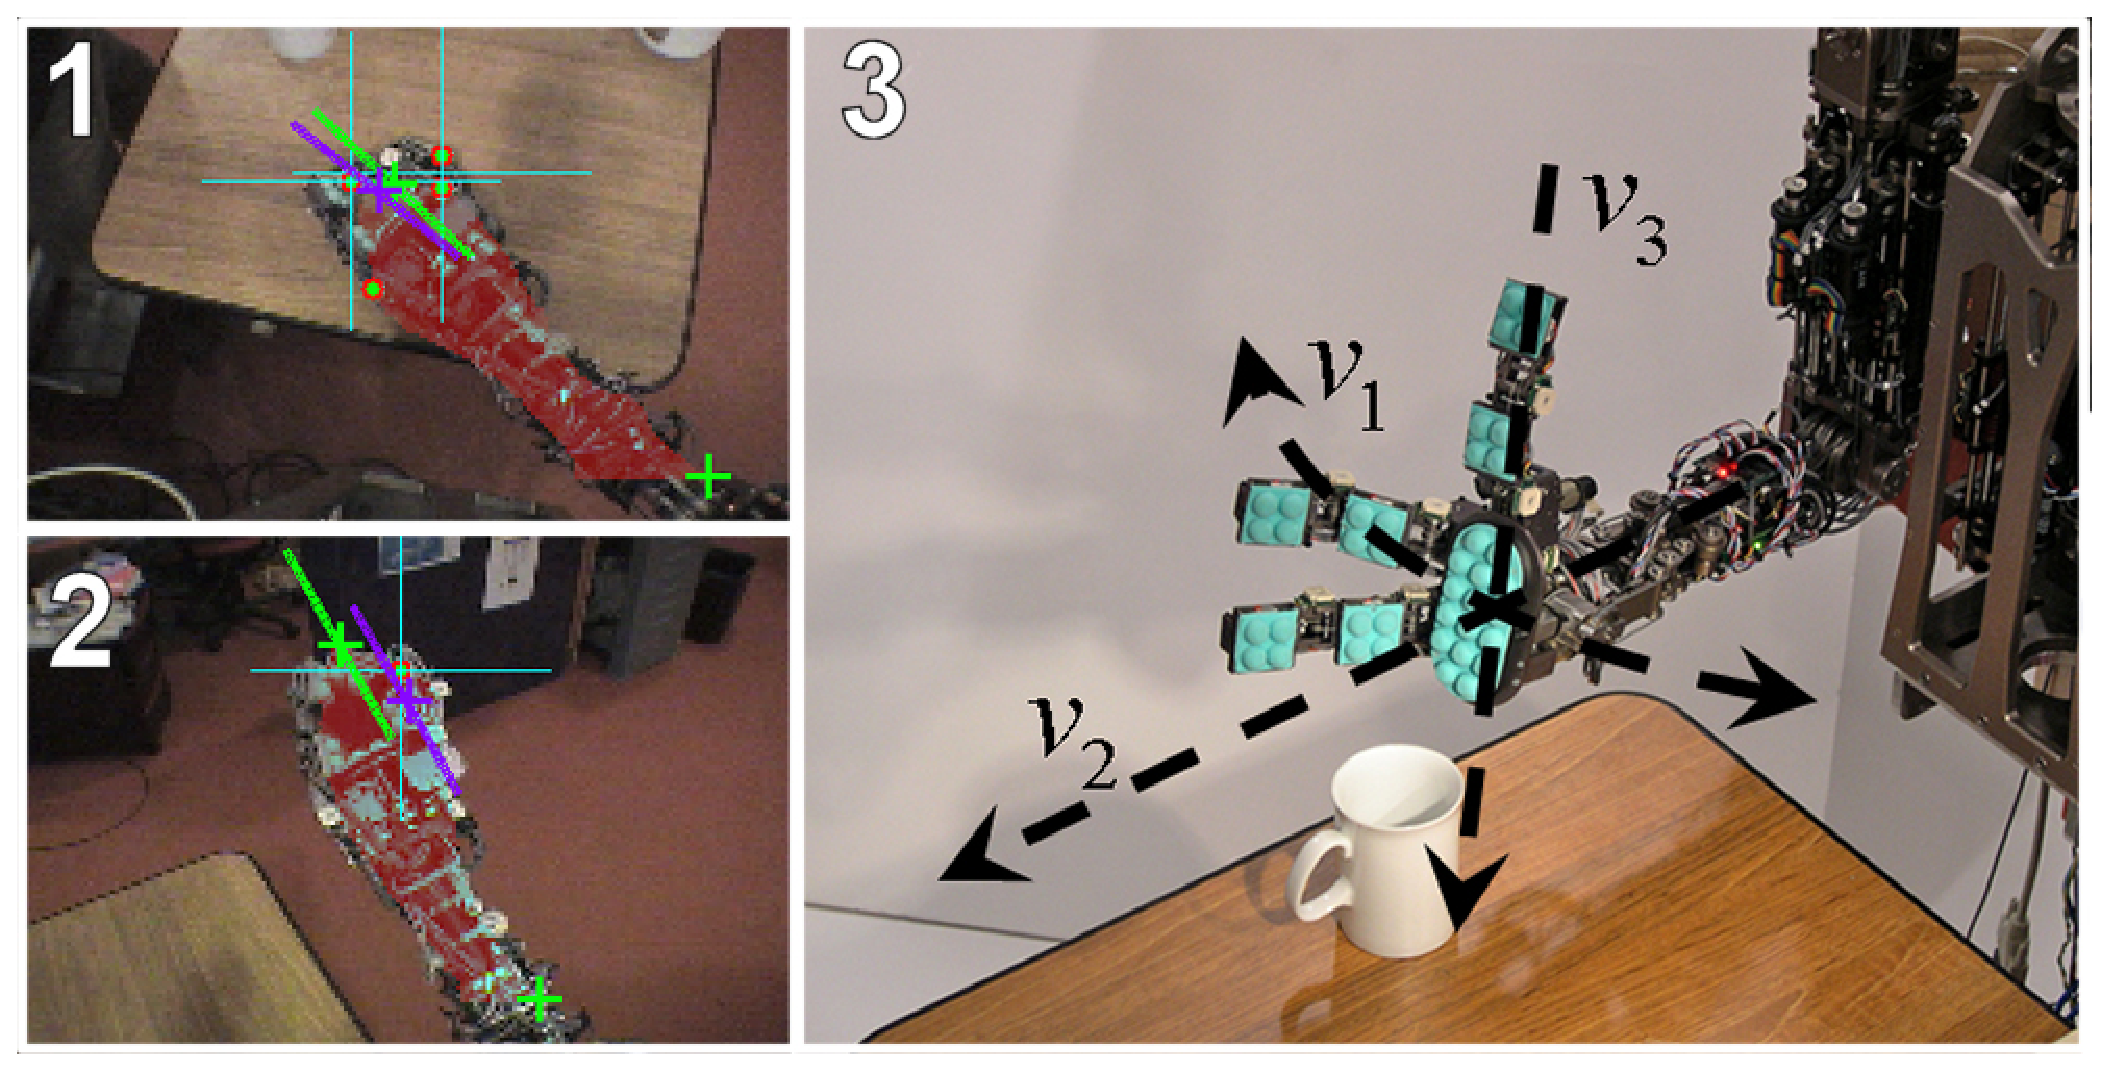
\includegraphics[width=\columnwidth, angle=0 ]{./figures/expl-directions.eps}
  }\caption{Left, frames 1 and 2: hand localization and arm
    orientation. Right, frame 3: exploration primitives. Primitives $v_1$
and $v_2$ are perpendicular and parallel to the arm orientation.
$v_3$ is along the null space of the arm Jacobian. These primitives
are sketched here in the cartesian plane for simpler understanding, but 
they are actually computed in the joint space (see 
Section~\ref{sec:controlling} for more details.}
\label{fig:expl-directions}
\end{figure}
%
\subsection{Exploration}
Starting from the direct mapping of the hand position and arm orientation we
can identify a set of explorative primitives, that is a set of vectors in
joint space that allows the robot to explore the arm workspace. We chose three
vectors $v_1$, $v_2$ and $v_3$, as follows (see also 
Figure~\ref{fig:expl-directions}):

$v_1$: moves the hand along the
direction perpendicular to the arm. It is computed by planning a 
reaching movement towards a point a few pixels away from the hand along the
line perpendicular to the orientation of the arm.

$v_2$: moves the hand along the
direction of the arm. It is computed by planning a 
reaching movement towards a point a few pixels away from the hand along the 
arm.

$v_3\in \ker \left(J\left(q_{arm}\right)\right)$: $v_3$ lays in the null 
space of the arm Jacobian; in our case the null space of the Jacobian 
consists of those vector that do not affect
either the projection of the hand onto the visual plane or the orientation
of the arm. These vectors produce a movement of the hand along the optical
axis of the camera, or, in other word, along $R$.
%
\subsection{A grasping behavior}
In this section we describe the grasping behavior of the robot.
The sequence begins when the experimenter waves an object in front
of the robot. The head tracks the object until it remains
stationary within the workspace of the arm. The robot reaches for
the object; motion is planned visually as described in
Section~\ref{sec:reaching}. Reaching is not accurate enough to
guarantee a correct grasp. Since no three dimensional information
is available the arm reaches a region above the object (see
Section~\ref{sec:reaching}). At this point the exploration starts;
the robot computes the explorative primitives $v_1$, $v_2$ and
$v_3$. The exploration uses three behaviors: 
%
\begin{itemize}
\item \emph{hovering behavior}, moves the hand back and forth along 
$v_1$.
%
\item \emph{pushing behavior}, moves the hand
along $v_2$.
%
\item \emph{depth behavior}, moves the hand ``downwards''
along $v_3$; this behavior moves the hand along the direction of
the optical axis of the camera and adjusts the height of the hand
with respect to the object/table. To avoid crashing the hand into
the table this behavior is inhibited when the infrared proximity
sensor detects an obstacle (usually this happens close to the
table).
%
\end{itemize}
%
The \emph{hovering behavior} and the \emph{depth behavior} are
activated at the beginning of the exploration. The goal of this
initial phase is to adjust the position of the hand until the
index finger touches the object. This allows adjusting the
position of the hand along the directions $v_1$ and $v_3$. During
the exploration the arm stops when the hand detects the object, to
avoid pushing it away or knocking it over; if no contact is
detected, on the other hand, the amplitude of the exploration is
extended (this increases the probability to touch the object in
case the reaching error is large). The exploration terminates when
the contact with the object is detected by any of the tactile
sensors placed on the index finger. At this point the \emph{hovering
behavior} is suspended and the \emph{pushing behavior} activated. The
``pushing'' movement along $v_2$ brings the palm in contact with
the object while the \emph{depth behavior} takes care of
maintaining the correct distance with the table. When the robot
detects contact on the palm the exploration stops and the
\emph{grasping behavior} is activated. The \emph{grasping
behavior} simply closes the fingers to a specific position. The
low impedance of the joints allows the fingers to adapt to the
different objects being grasped.

Figure \ref{fig:sequence} reports an example of the robot grasping 
a porcelain cup. The grasping behavior proved to be quite reliable, as 
repetitive tests show in Section \ref{sec:results}
\section{Results}
\label{sec:results}

\begin{table*}[tb]
  \caption{Objects} \label{tab:objects} \centering
  \begin{tabular}{|c|l|c|c|c|l|}
    \hline
    &Description& Weight(Kg)&No.Trials&No.Failures&Contains \\
    %&Object& W(Kg)&Trials&Fail&Contains \\
    \hline
    1&White Bottle        & 0.265 & 22& 0 & Vitamins\\
    2&White Porcelain cup & 0.255 & 24& 1 & Nothing\\
    3&Startbucks cup      & 0.220 & 24& 4 & Bolts \\
    4&Nesquick box        & 0.240 & 24& 2 & Nesquick powder\\

    \hline
  \end{tabular}
\end{table*}

\begin{figure}[tbp]
\centerline{
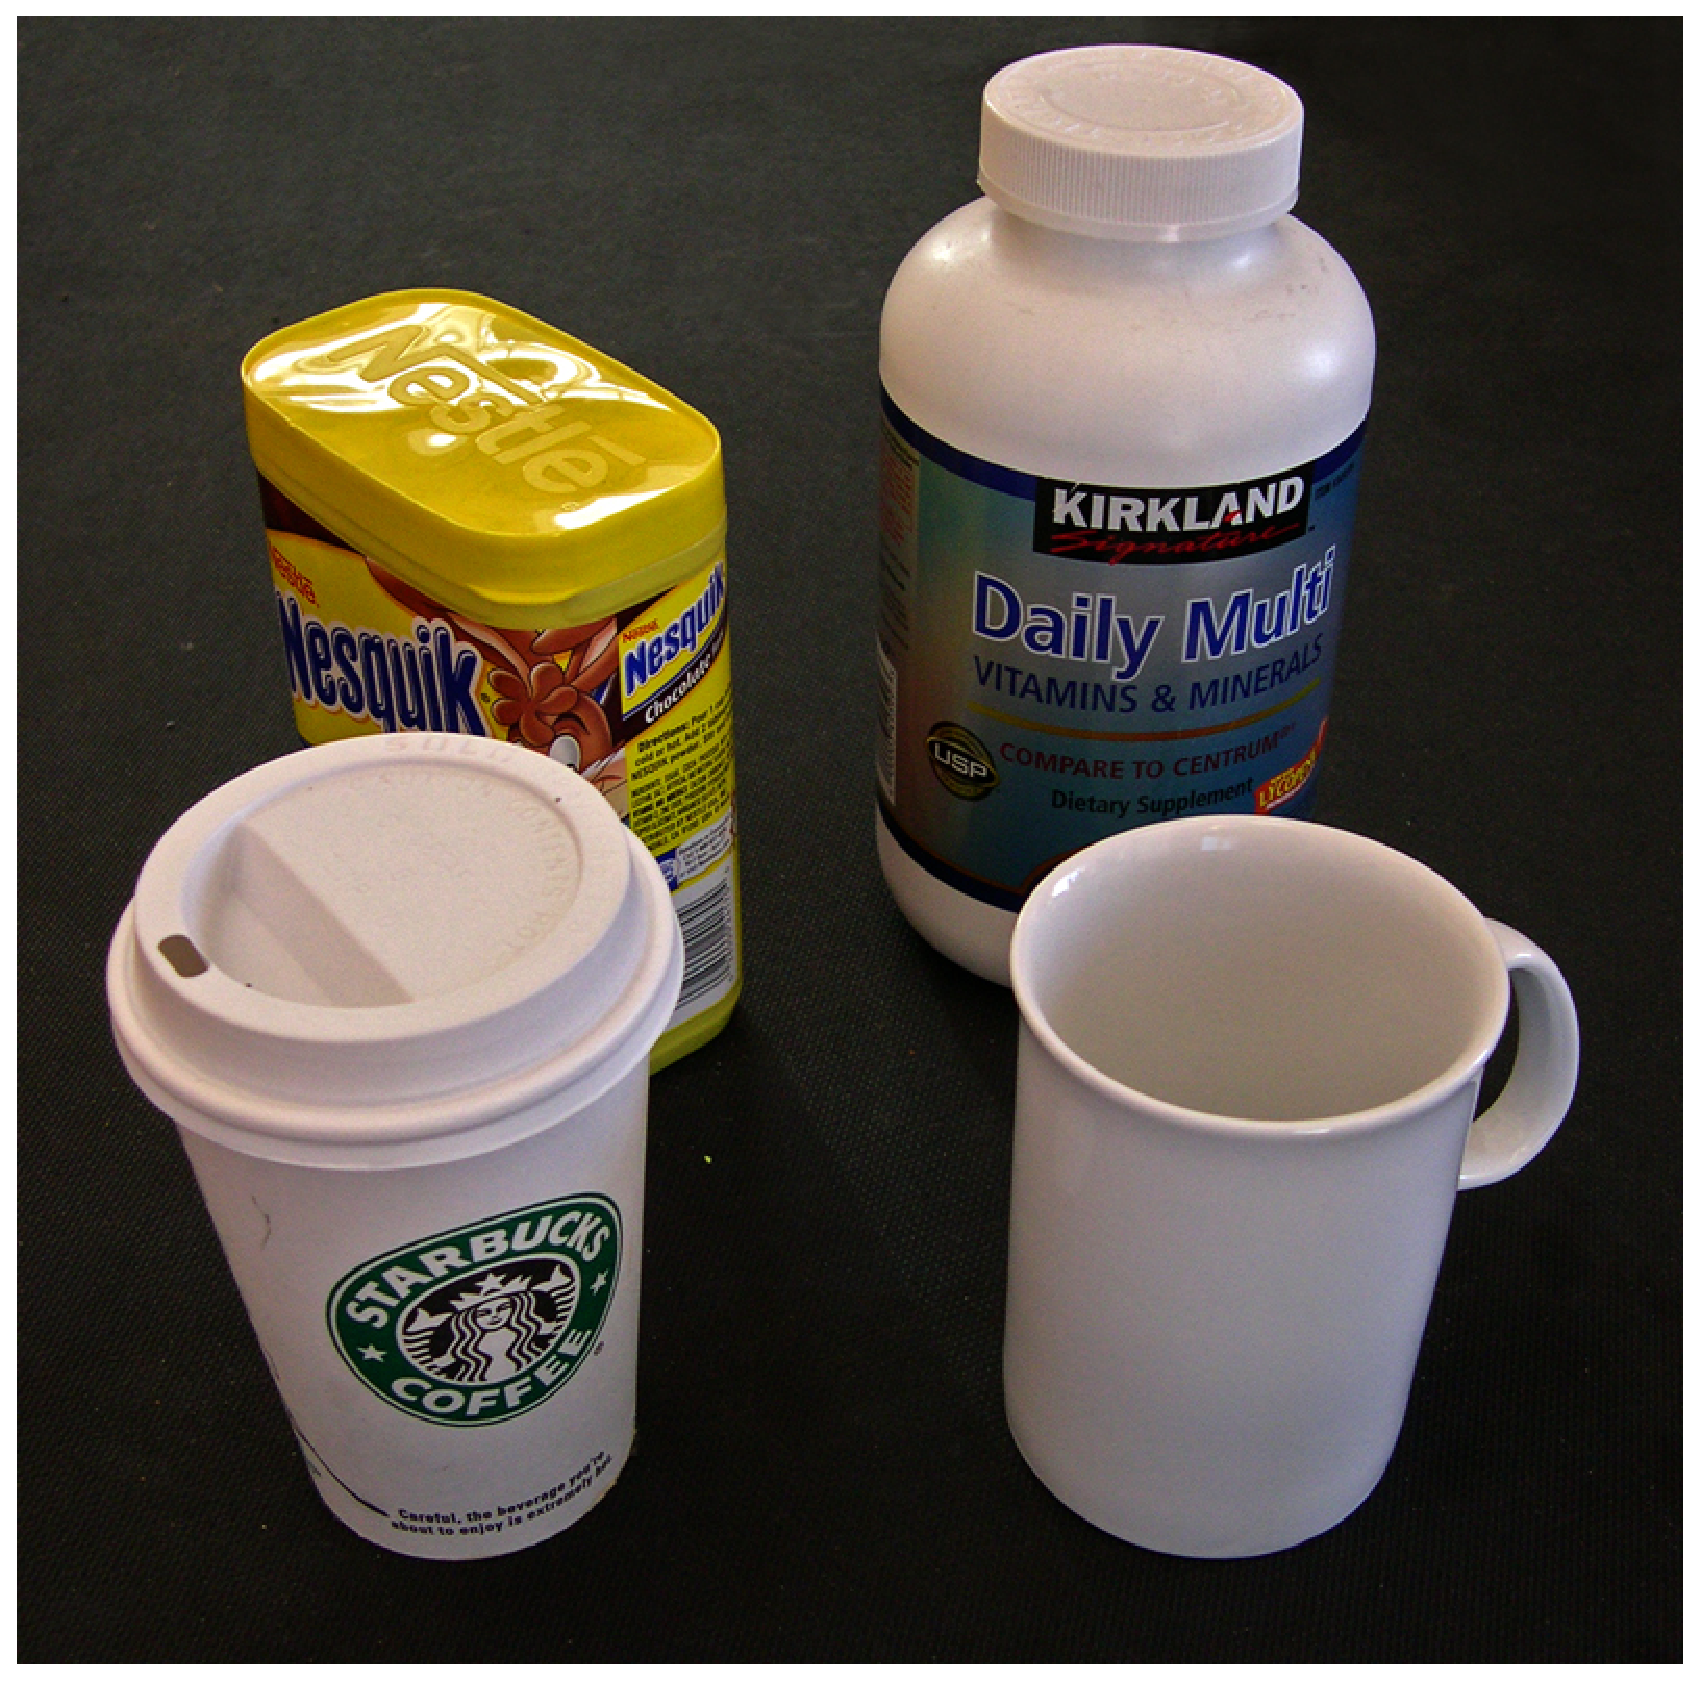
\includegraphics[width=2.0in]{./figures/objects.eps}
}\caption{Objects}
\label{fig:Objects}
\end{figure}

An example resulting from the implementation described in
section~\ref{sec:behavior} is shown in figure~\ref{fig:sequence}.
We can observe the reaching action followed by the positioning and
grasping. [Should we include a plot of the readings of the
sensors?]


Using the behavior described in section~\ref{}, the robot was able
to grab a number of different objects. The robot had no prior
knowledge of the objects. We evaluate the performance by
presenting to the robot many times four objects and counting the
number of times that they were grabbed. Out of 94 trials only 8
failed. The objects were : a white vitamins bottle, a white
porcelain cup, a startbucks cup and a nesquick box. The physical
properties of the objects and the results are shown in table
\ref{tab:objects}.

[No sure if we should include this part]

We have also evaluated the behavior of the tactile sensor grabbing
the same object but with different weights. The object used was
the white bottle and the weights used are presented in the
table~\ref{}.






%We evaluated our work by performing an object recognition
%experiment. We exposed the robot one evening to a set of seven
%objects, and then in the morning tested its ability to recognize
%another set, which had an overlap of four objects with the
%training set. Three of these objects were chosen (Figure 8) to
%represent three different materials, plastic, glass and steel
%(metal). The idea is that the sound produced by each object
%depends on its size, shape and the material with which it is made;
%accordingly we expected the tapping to produce three different
%distinct sounds. A fourth object (a plastic toy) was relatively
%silent. For each run, we placed randomly selected objects on the
%table in front of the robot, and it was responsible for finding
%and tapping them. Overall the robot tapped 53 times; of these
%episodes 39 were successful, meaning that the sound produced by
%the tapping was significantly loud; in the other 14 cases the
%tapping did not provoke useful events either because the initial
%impact caused the object to fall, or the object remained too close
%to the hand. The high number of successful trials shows that given
%the mechanical design of the hand, haptic feedback was sufficient
%to control the interaction between the robot and the environment.
%We evaluated the performance of our spectrum comparison method by
%ranking the strength of matches between episodes on the second day
%and episodes on the first day. Figure 7 shows what detection
%accuracy is possible as the acceptable false positive rate is
%varied. This predicts that we can on average correctly match an
%episode with 50\% of previous episodes involving the same object
%if we are willing to accept 5\% false matches.

\section{Conclusions}
In this paper we have described the implementation of a reaching
behavior that integrates together an open loop and a closed 
loop controller. The open loop controller
allows the robot to perform faster movements and does not require visual 
feedback from the hand. When sight of the hand is available the closed
loop controller allows for precise positioning of the hand in the 
image plane. The procedure among the other things estimates the eye-to-hand
visual Jacobian of the robot. In this respect our method provides
similar results to the ones described in the literature \cite{}

We describe an explorative strategy by which the robot autonomously 
acquires the transformations required to control the hand to reach for a
visually identified target.

We do not rely on any prior information about the 
parameters of the robot. The only simplification was that we used 
a color mark to visual localize the hand of the robot. Our assumption
is that the hand localization/identification is a separate problem
that needs to be solved before learning reaching. Previous work
by the same and other authors have suggested procedures by which 
the robot could autonomously learn to solve this task 
(\cite{Natale05,edsinger06what}). It will be interesting to see
how these approaches can be integrated with the work described 
in this paper.

\section*{Acknowledgements}
This research benefited from discussion with Giorgio Metta. 
The authors would like to thank Paul Fitzpatrick, Charles Kemp 
and Lijin Aryananda for providing some useful code. Funds for this 
project were provided by ABB, by the NASA Systems Mission Directorate,
Technical Development program under contract 012461-001, by 
DARPA DABT 63-00-C-10102, and by NTT under the NTT/MIT Collaboration 
Agreement. Lorenzo Natale was supported in part by the European Union 
grant RobotCub (IST-2004-004370).




%  Generate ``References'' here.
\bibliographystyle{sab}
\bibliography{natetorresj}

\end{document}
